\documentclass{standalone}

\usepackage{placeins}

\begin{document}
	Throughout the following chapter, we shall analyse the intricate specifications of our application and accordingly propose sensible design solutions. This will consist of describing the application as a whole, then delving into each of the individual aspects. By the end, the reader should obtain a strong understanding of what exactly our application does along with the utilised core techniques.

	\section{Software Development Process}
		Firstly, we shall describe the overall methodology and workflow that have been employed throughout the duration of development. These are of important consideration as they promote both an effective and productive approach to the creation of software. Much of what is to be described is inspired by the ideas expressed in \parencite{pragmaticProgrammer}.

		As the application is not a collaborative undertaking, there is little-to-no need in sticking strictly to any specific paradigm or framework for the software development process; as it would most probably lead to unnecessary overhead and distraction from any relevant progress. However, it is still of purpose to state that development most closely resembles the set of principles described under Agile \parencite{beck2001agile}, in that the application's design and implementation occurred concurrently, with continuous adaptation.

		Over the course of the development process, the Git \parencite{gitWeb} version control system has been used to track file changes. Among other benefits, this allows us to maintain a full history of our application's source code, enabling us to revert back to previous versions - removing undesired changes. To further the backup capabilities, the Git repository is hosted online at GitHub\parencite{TronGitRepo}.

		In order to manage the various short-term goals throughout development, a todo-list (in the form of a plaintext file) has been maintained. The purpose of which was to help maintain an efficient workflow and provide a medium for documenting design thoughts between development sessions.

		To aid future developers, or those studying the application, all source-code has been passed through a lint utility. This helps to identify potential bugs and preserve a consistent coding standard - by identifying syntactic discrepancies. Also, the source code itself contains extensive documentation; in the form of both relevant variable names and comment annotations.

		\subsection{Package Scripts}
			We have also assembled a repertoire of scripts that serve the purpose of automating some of the tedious tasks which are executed on a regular basis. In abstracting away from these laborious procedures, we have reduced the chance of unnecessary complications whilst also improving the efficiency of working with the application.

			Below is a curated list of the available scripts, along with a short description of their purpose.\footnote{Also, when a developer attempts to push to the GitHub repository, our unit-test are automatically performed; aborting the push upon failure.} However, please mind that some reflect ideas we have yet to discuss. (for more detail, please see \fullref{sec:reactUniversally})
			\begin{formal}
				\begin{lstlisting}[language=bash,style=codefigure,
caption={Creates an \texttt{webpack-bundle-analyze} session against the production build of the client bundle.}]
yarn run analyze:client
\end{lstlisting}

\begin{lstlisting}[language=bash,style=codefigure,
caption={Creates an \texttt{webpack-bundle-analyze} session against the production build of the server bundle.}]
yarn run analyze:server
\end{lstlisting}

\begin{lstlisting}[language=bash,style=codefigure,
caption={Builds the client and server bundles, with the output being optimized.}]
yarn run build
\end{lstlisting}

\begin{lstlisting}[language=bash,style=codefigure,
caption={Builds the client and server bundles, with the output including development related code.}]
yarn run build:dev
\end{lstlisting}

\begin{lstlisting}[language=bash,style=codefigure,
caption={Deletes any build output that would have originated from the other commands.}]
yarn run clean
\end{lstlisting}

\begin{lstlisting}[language=bash,style=codefigure,
caption={Deploys your application to \href{https://zeit.co/now}{\texttt{now}}.}]
yarn run deploy
\end{lstlisting}

\begin{lstlisting}[language=bash,style=codefigure,
caption={Starts a development server for both the client and server bundles.}]
yarn run develop
\end{lstlisting}

\begin{lstlisting}[language=bash,style=codefigure,
caption={Executes \texttt{eslint} against the project.}]
yarn run lint
\end{lstlisting}

\begin{lstlisting}[language=bash,style=codefigure,
caption={Executes the server. It expects you to have already built the bundlesusing the \texttt{yarn run build} command.}]
yarn run start
\end{lstlisting}

\begin{lstlisting}[language=bash,style=codefigure,
caption={Runs the \texttt{jest} tests.}]
yarn run test
\end{lstlisting}

\begin{lstlisting}[language=bash,style=codefigure,
caption={Runs the \texttt{jest} tests and generates a coverage report.}]
yarn run test:coverage
\end{lstlisting}
			\end{formal}

	\section{General Design}
		The application itself is quite a large undertaking, as it comprises a multitude of different aspects. Most of which can be categorised into one of three groups: game mechanics, network communications, and artificial intelligence. Therefore, where possible, we shall try to discuss each one of these categories separately. But first of all, we shall introduce the reader with an overview of the application and describe the relation between some of its core components.

		\subsection{Architecture Overview}
			Much of what has been designed is derived from ideas that relate to the game as a whole, that being the overall encompassing architecture. To aid the reader in understanding said content, we shall introduce them to a brief summary of the foundational ideas in which the game is to be built upon.

			At its heart, the game follow a client-server multiplayer game architecture. This is where a single device is designated to be responsible for processing user-input, updating the game state and communicating said game state to the connected players. The connected players are principally responsible for relaying input to the server and rendering graphics based upon the state communicated from the server.

		\subsection{Core Technologies}
			As the game is to be played in a web-browser, we will be making use of the three fundamental web languages; HTML, CSS, and JavaScript. These three languages, and the standards which govern them, allow us to confidently write portable code which will run predictably within the majority of web-browsers. Although, sadly this is not always the case as it is notorious for many web-browsers to not always fully support the most up-to-date standard - assuming it follows it in the first place.

			The primary programming language for our client-side source-code is JavaScript; the standard core web-browser technology for DOM manipulation of a web-page. To help tackle the compatibility issue mentioned above, the all our JavaScript will conform according to the ECMAScript2015 standard \parencite{ECMAScript2015}. It shall then be transpiled to a more universally supported syntax using Babel \parencite{Babel}.

			Transpiling to JavaScript has become somewhat the norm in the realm of modern web-development. In recent years, many entirely new programming languages have emerged for the sole purpose of being transpiled into JavaScript. For this application, the decision to use an updated standard of JavaScript, as opposed to one of these entirely new languages, is to reduce the amount in which we abstract from the underlying code that is to be executed; removing another layer where issues could arise.

			As our game is designed to be played within a web-browser, we already have access to the wide range of graphical components and other features described within the HTML specification. Notably, this includes elements such as buttons, lists, hyper-links and CSS - which is used to describe the presentation of our web-document.

			As the logic and state of our game exists within JavaScript, we will need to frequently manipulate these HTML elements - such that a proper reflection of our game state is maintained. This type of structure closely resembles the Model–view–controller \parencite{MVC} software architectural pattern for implementing user interfaces. However, handling the view layer can prove to be quite a cumbersome task as many naive solutions scale very poorly, such that future adjustments may have adverse side affects or may just be very awkward to implement; making correctness difficult to conserve.

			\begin{figure}[!htbp]
				\centering
				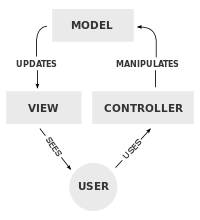
\includegraphics{resources/images/mvc.png}
				\caption{Diagram depicting the Model–view–controller software architectural pattern, from \parencite{MVC}.}
			\end{figure}

			\label{redux}
			Thankfully, this is a very common problem faced during web-development, and there already exist many capable candidate solutions. With this in mind, along with the desire to learn a new framework, and the curiosity regarding its applicability in integration with this project; React\parencite{React} and Redux\parencite{Redux} have been employed to help manage the view layer.

			React is a popular JavaScript framework that makes it relatively easy to create advance user-interfaces for web-applications. It allows you to design your application as a set of simple views for each state in your application, and will efficiently update and render only the appropriate components when data changes. In essence, this is done by constructing almost your entire application's view layer within JavaScript by building encapsulated components - each charged with managing their own state.

			Redux is a separate library, but plays very well when used in conjunction with React. Simply put, it is a predictable state container for JavaScript applications. It aids in allowing the developer to write application that behave in a consistent manner, whilst providing tools to improve the developer's experience in regards to processes such as debugging.

			Redux, in principle, requires the application's state to be stored in an object tree inside a single data \emph{store}. Each state is represented by a single immutable object. Changes to the state tree are made by emitting \emph{actions}. An \emph{action} is an object describing what happened during some event to the state. These \emph{actions} are then used to transform the state tree through the use of \emph{reducers}; a pure function, with \texttt{(state, action) => state} signature, describing how an action transforms the given state into the next state.

			Given that we already have to use JavaScript for our front-end game code, it makes sense to not bring in another language for our back-end. This bears a myriad of benefits, such as not having to deal with the additional quirks of a separate programming language. Also, it eliminates the hassle of maintaining two separate implementations of code that is identical in purpose. This becomes especially relevant later on, when we introduce client-side prediction (see \fullref{clientPrediction}). Hence for the back-end, that is the code which will be executed on a dedicated server, we shall be utilising Node.js\parencite{NodeJs}.

			Node.js, is a technology which serves as a JavaScript runtime environment allowing JavaScript to run in standalone, outside of a web-browser. It has become a major proponent of the \enquote{JavaScript everywhere} paradigm, allowing the meat of web-application development to unify around a single programming language. A concise description is provided on the front-page of its website:
			\begin{formal}
				\enquote{Node.js® is a JavaScript runtime built on Chrome's V8 JavaScript engine. Node.js uses an event-driven, non-blocking I/O model that makes it lightweight and efficient.} - \cite{NodeJs}
			\end{formal}

		\subsection{Boilerplate}
			\label{sec:reactUniversally}
			Somewhere early on during development, having already settled on the aforementioned technologies, it began more and more difficult to maintain an efficient development workflow. That inspired the decision to transition the project to the use of the React Universally \parencite{ReactUniversally} starter-kit; a boilerplate project with a bare-bones base structure along with various scripts to help automate the tedious build/watch transpile process required for our JavaScript code.

			React Universally also sets up Server-side rendering with React. This is helpful as it enables the server to perform an initial render of our application's components, then serve the result to the client. This results in the web-page appearing to load faster, as the main layout would've been pre-rendered; so the client user does not experience the initial flickering of DOM elements as the view is mounted.

			Regarding the Redux store, the state is simply injected directly into the web-document prior to being served to a client. Upon initialisation, the client immediately rehydrates the application using the transmitted state and mounts the React components.

			The source code directly composing our application is split into three main directories: \emph{shared}, \emph{client}, and \emph{server}. The \emph{shared} directory contains the bulk of our application, including source which is rendered server-side to be served to a client. Whilst the \emph{client} directory is for browser specific source that is not to be used server-side, not even for the purpose of server-side rendering. In particular, it includes functionality such as user-input and establishing a live communication session with the server. In a similar respect, the \emph{server} direction contains all the source specific to our Node server.

	\section{Game Mechanics}
		Compared to other arcade games, Tron has relatively few fundamental game mechanics. However, with that being said, there are still many challenges that arise due to the game's fast-paced nature and critical requirement for accuracy. Throughout this section, we shall discuss some of the more integral problems regarding the game's core mechanics along with the designed solutions, and the techniques in which they use.

		Before we delve into the specifics, it is vital we first provide an overview of the game's state object. In video-game design, the game state refers to an object - or other data store - which contains all the data representing a game instance at some particular point in time.

		Below is a breakdown our game state object's structure:
		\begin{description}
        \item[tick]: the number of times this state has ticked; inclusive of the current tick update.
        \item[progress]: the amount of time which has passed since the last tick update.
        \item[started]: a boolean indicating if a round of Tron is in progress.
        \item[finished]: a boolean indicating if the current round has finished. \emph{undefined} if started is \emph{false}.
        \item[arenaSize]: the number of cells within our game arena.
        \item[playerSize]: the number of cells a player occupies within our game arena.
        \item[speed]: the number of cells each player travels over the course of a millisecond.
        \item[players]: an array containing an object for each player part of the current game. The following describes the structure of a single player object:
        \begin{description}
        	\item[id]: a unique string used to identify the player.
        	\item[name]: an arbitrary string for other players to recognise this player.
        	\item[alive]: a boolean indicating if the player is alive, or otherwise dead.
        	\item[direction]: the direction (north, south, east, or west) in which the player is travelling.
        	\item[position]: a \emph{point} (an array, in the form of [\emph{x, y}]), representing the player's current position in the grid.
        	\item[trail]: an array of \emph{points} at which the player has changed direction. Used to construct a path of the area in which the player has travelled. However, the array has two special cases: the first element is the player's spawn point, and the last element is the point for the player's previous position.
      	\end{description}
        \item[cache]: a nested object containing various cache structures required by our state. The following describes the structure of the cache object:
        \begin{description}
        	\item[collisionStruct]: a data-structure in which we can check for player/trail collisions within our arena. See for more detail \fullref{collisionDetection}.
      	\end{description}
    \end{description}

		Our game state itself must be implemented as a mutable object. This is due to the large overhead that immutability generates; primarily from computationally expensive processes, such as copying an abstract data-type. As immutability is optional, it therefore is simply not worth introducing it within the game loop - as it would degrade performance.

		Although having the game state be a mutable object does not directly interfere with our server, it does raise concern in regards to our client and their utilisation of Redux. This is because one of Redux's key principles, is that all data held within the \emph{store} must be immutable, such that all modifications to the state are performed solely by \emph{reducer} functions.

		To avoid creating an unnecessary reliance and coupling of the project onto optional technologies, we do not want to meld our internal game code with Redux. Hence, for our client, when we receive a game state update from the server we copy it and commit both the original and copy into the \emph{store}. One of these stored game states will remain immutable, whilst the other will be fully mutable - hence unaware of updates.

		This solution may currently appear rather strange, as at this stage it is too early to introduce the entire reasoning reasoning. However, simply put, it allows us to keep an authoritative state (what is known) and a predictive state (what should be). Our DOM will reflect the authoritative state, whilst the drawn graphics of the game will reflect the predictive state (for more information, see \fullref{sec:lagCompensation}).

		The next major aspect of our game is the game loop. In principle, it is a section of code that runs continuously during game-play, at some interval. User input is processed, without blocking, during each \emph{tick} of the loop. The remainder of the \emph{tick} is then used to update the game's state and render graphics. It of critical importance, and is arguably the most employed pattern in game-design as it provides a very convenient and deterministic way in which the developer can structure their game.

		Our game shall be utilising the game loop, and is heavily based around said pattern. In principle, the server needs to spin the game loop at a rate fast enough to process user-input and calculate updates without introducing noticeable latency. Whilst the client is only required to spin fast enough to create the illusion of animated graphics.

		By default, both client and server will have their game loop configured to run at a tick-rate of once every 15 milliseconds - approximately 66 times a second. \footnote{This is considered the standard for video-games. In most cases, any faster rate does not have much of a distinguishable benefit.}

		\subsection{Collision Detection} \label{collisionDetection}
			Many existing Tron implementations internally use a grid-based arena, that is a play occupies an entire whole cell of the arena. This enables collision look-ups to be performed in constant time, by simply indexing an array. However, our implementation allows players to move with an incredibly high-degree of precision\parencite{JsNumbers}. Unfortunately, this does complicate collision lookups.

			Instead of checking for collisions against every object in the arena, we have utilised the uniform grid spatial data-structure. This allows us to divide the arena into a grid of arrays, where each array holds references to the objects that reside within its bounded space. Thus, when checking for a collision, we only need to check against objects that are held within the array(s) that our target object intersects with; reducing the search space quite substantially.

			To populate our collision data-structure, we generate a series of rectangles representing each individual line-segment that forms the player's trail - from their current position, to the position they were spawned at. This is the stage at which we take into account the players' size.

			\begin{figure}[!htbp]
				\centering
				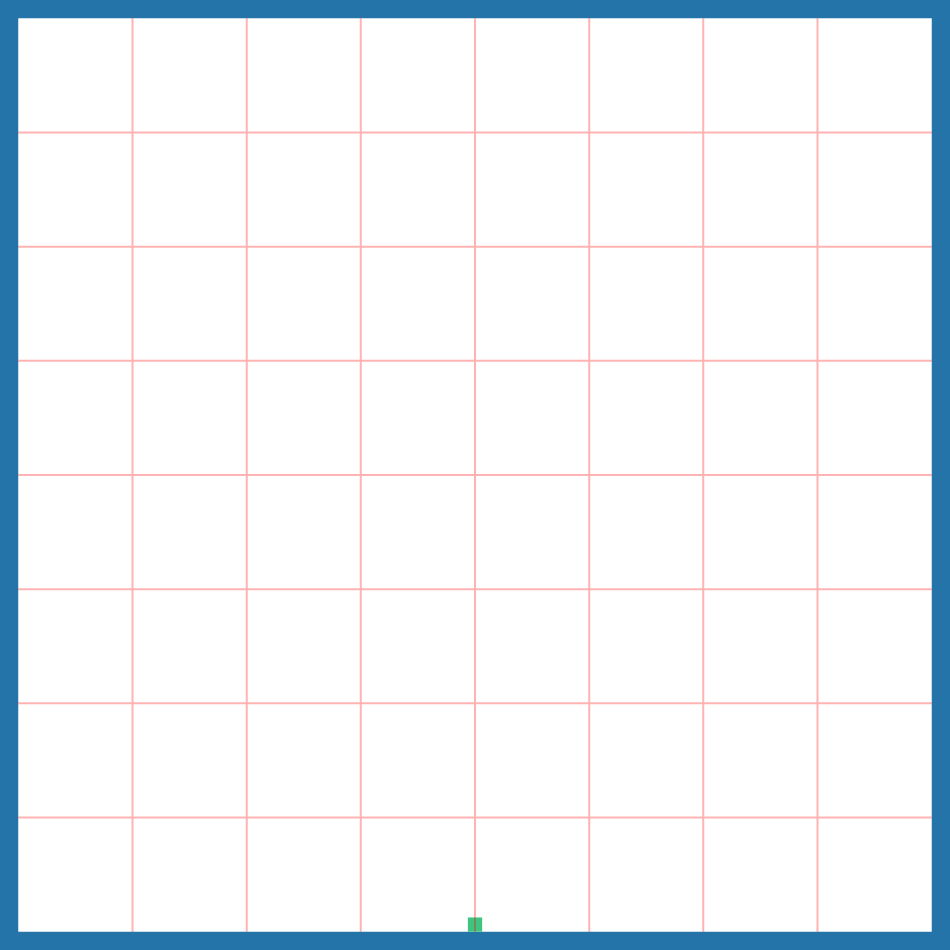
\includegraphics[width=.8\textwidth]{resources/images/uniformgrid.png}
				\caption{Visualisation of uniform-grid data-structure, drawn by our game's draw debug mode.}
			\end{figure}
			\FloatBarrier

			Once the search space has been reduced, we now need to check to see if any of the obtained objects collide with our target object. Conceptually, this is just checking if there exists an overlap between two rectangles; a very simple calculation. However, as we want players to stop at the precise moment at which they crashed, we must calculate the intersection point and then offset it appropriately using the size of the two players.

			This boils down to two distinct cases: \footnote{Please note that, in our collision case diagrams, the black dot within a player represents their position point. \label{blackDotDiagram}}
			\begin{enumerate}
    		\item
    			\textbf{Case}: player collides with another player - who is not heading in an opposing direction.\\
					\textbf{Solution}: reposition the crashed player by appropriately calculating an offset distance from the player they hit - based upon both their sizes. Using the crashed player's travelling direction for the offset's sign. \\
					\begin{minipage}{\linewidth}
						\centering
						\captionsetup{width=.8\linewidth}
	          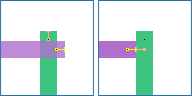
\includegraphics[width=.8\linewidth]{resources/images/collision/side.png}%
	          \captionof{figure}{Example of a sideways collision. On the left, two players are depicted in their unfixed positions. Whilst on the right, they're now shown in their relative position.}
	    		\end{minipage}
				\item \label{itm:headCollision}
					\textbf{Case}: head-on collision between two players.\\
					\textbf{Solution}: move each player backwards by half the sum of their \emph{overlap} and \emph{overshoot}.\\
					\begin{minipage}{\linewidth}
						\centering
						\captionsetup{width=.8\linewidth}
	          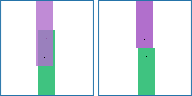
\includegraphics[width=.8\linewidth]{resources/images/collision/headon.png}%
	          \captionof{figure}{Example of a head-on collision. On the left, two players are depicted in their unfixed positions. Whilst on the right, they're now shown in their relative position.}
	    		\end{minipage}
			\end{enumerate}

	\section{Network Communication}
		\label{gameLobby}
		For a game to be multiplayer, all players need to share the same consistent experience across a network, i.e. they need to all be playing on the same game state. So this raises the question on how to synchronise the game state between all connected players. There are two main methods to achieve a synchronised game state and, to some degree, we will be using ideas from both.

		The first method is known as \emph{peer-to-peer lockstep}. It centres around the idea of the game being modelled as turn-based and, before each turn, all non-deterministic events (such as user-input) are broadcasted to all players. Once all players have sent their input for this turn, each player then individually updates their game state; which will of course all end up being identical. The primary flaw in this technique is that all players are forced to play at the latency of the player with the weakest connection. This would be extremely frustrating for Tron, as each time you try to move you have to wait for the player with the weakest connection.

		The second method is known as \emph{client/server}. It entails having a single authoritative game-state kept on a server, that is then communicated between all players. When a player wants to perform an action, they must communicate said action to the server. The server will then apply the action and communicate the updated state to all connected players. However, this solution makes no compromises for latency. For example, the server's state is forever being updated and it will often receive actions from connected players that were made under the assumption the game is still at some previous state.

		\label{clientPrediction}
		Our developed solution entails the use of several techniques. At its core, it is a client-server model. But we make use of two mechanisms known as \emph{lag compensation}\parencite{LagCompensation} and \emph{client-side prediction}\parencite{LagPrediction} which help to reduce the negative effects of latency.\label{sec:lagCompensation}

		Simply put, lag compensation enables the server to `rewind` time when applying the input of a user; compensating for any latency that may have occurred. Whilst lag prediction allows clients to mimic the server, including the immediate processing of their input. See \parencite{LatencyCompensating} for a more thorough description.

		Communicating the entire game state after each tick is an incredibly infeasible task; each player would be required to communicate with the server at a rate faster than the game's tick-rate.

		Our solution to this problem is quite a simple one. When the client receives a message containing the updated state, they immediately reply to the server with an acknowledgement. The server will interpret this acknowledgement as a request to prepare the next state transmission.

		To further reduce the latency of communication, we can also reduce the payload size of each state transmission. This is made possible by identifying that over the course of several ticks, the game state remains largely unchanged. Knowing this, we are able to keep in memory the last state communicated to each player and when we need to transmit, just calculate a snapshot of the differences \footnote{We calculate and apply the differences using \emph{fast-json-patch}\parencite{FastJsonPatch}.} between the current state and the last one which was sent. We also don't bother sending the cache, and instead simply regenerate it on the client - which isn't too expensive of an operation, and doesn't hinder our server's authoritative game state.

		\label{designCommunicationTechnologies}
		As introduced within the background section (see \fullref{sec:browserTechnologies}) there exist several technologies capable of handling the actual communication with a web-server; most notably Web-Sockets and Web-RTC. However, due to the use of a dedicated game-server running Node, Web-Sockets is our chosen communication technology.

	\section{Artificial Intelligence} \label{sec:design-ai}
		In order for our computer opponent to play the game, they need to be controlled by some artificial intelligence; some program which has an understanding of the game and can make sensible moves, as if it were a human player. This is quite a complicated, especially given that our game is played in real-time.

		Our solution to this problem centres around the idea of the modelling the game to be both played on a grid and turn-based, then running simulations which play out the possible scenarios in which the game could develop. However, as we require our AI to make decisions within a very short amount of time, we are unable to check the entire search-space and instead must make use of a variety of techniques to help optimise the process.

		Probably the most radical technique is to only run each simulation up until some fixed depth, at which point we then evaluate the current game state using an heuristic evaluation function. The effectiveness of this technique is heavily reliant on both the chosen fixed depth as well as the evaluation function.

		The heuristic evaluation function we've designed uses an optimised version of the flood-fill algorithm, featured in the very high-performing implementation that was the winner of a Google AI competition - introduced in \fullref{sec:background-google-ai}. The core idea is to count player \emph{ownership} of grid-cells, in our model of the arena, based upon a heuristic distance measurement.

		First, all players have their heuristic score initialised to 0. Then we calculate the minimum Manhattan distance between the AI player and all other alive players. We then apply flood-fill to calculate the distance from the current player to each empty grid-cell. Flood-fill is optimised by halting its process once the distance surpasses the previously calculated minimum distance. We are now left with a heuristic distance measurement.

		For each grid-cell, we then apply the following process to score based upon cell ownership: for each player, increment 1 to their score for every other player that has a distance that is greater-than, or equal to, the current cell. If the other player does not have a recorded distance to the current cell, instead increment by 2.

		Thus, a greater score indicates a stronger position; although not relative to other players.

		Even with the reduction in search-space and optimised evaluation function, time is still limited. So, we use Monte Carlo tree search \parencite{MonteCarloTreeSearch} with UCB1 to only explore promising branches of the game tree. 
		\begin{figure}[!htbp]
			\centering
			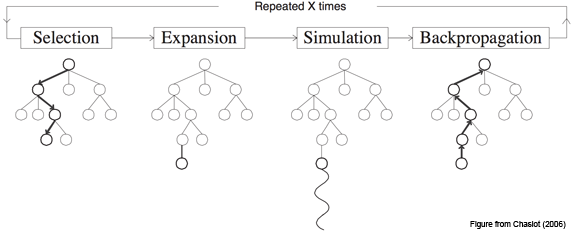
\includegraphics[width=.8\textwidth]{resources/images/mcts.png}
			\caption{Diagram depicting the Monte Carlo tree search algorithm, from \parencite{MonteCarloTreeSearchDiagram}.}
		\end{figure}

		On top of all of this, the simulations involved in calculating the artificial intelligence's move run in parallel to the rest of the game-server. This is done by spinning off a child process, which will run on a separate core. Once a move has been calculated, it will communicate the result back to the server and then die.

		The server will then apply lag compensation, once it receives the communicated move. This effectively allows simulations to take longer than the duration of a single tick; leading to moves that are generally better.
\end{document}